\section{Model and Problem Formulation}
\label{sec:formulation}

% 迁移自 docs/formulation.md；符号修正已应用：候选路径数 kappa，demand 集合 \mathcal{K}^t

\subsection{Network and Traffic Model}
\label{sec:model}

We model the constellation at control epoch $t$ as a directed graph
$G^t = (V, E^t)$, where $V$ is the set of $N$ satellites and $E^t$ the set of
inter-satellite links (ISLs), each link $e$ with capacity $c_e$. Time is
slotted into control epochs; within an epoch the topology snapshot is fixed,
while across epochs both $E^t$ and the traffic change as satellites move.

Traffic is described by a demand matrix $D^t \in \mathbb{R}^{N \times N}$,
where $d_i$ denotes the volume of the $i$-th source-destination pair. Since
satellite traffic is geographically concentrated, we maintain an \emph{active
demand set} $\mathcal{K}^t$, the pairs with nonzero demand in recent
history, and only these are modeled. Each demand
$i \in \mathcal{K}^t$ is served by $\kappa$ pre-selected candidate paths
$P_i = \{p_{i,1}, \ldots, p_{i,\kappa}\}$ ($\kappa = 4$ edge-disjoint
shortest paths in our implementation). The TE decision for demand $i$ is a
split-ratio vector $r_i \in \mathbb{R}^{\kappa}$ with $r_{i,k} \ge 0$ and
$\sum_k r_{i,k} \le 1$, allocating flow $f_{i,k} = r_{i,k} \cdot d_i$ to path
$p_{i,k}$; the residual $1 - \sum_k r_{i,k}$ represents intentionally
unserved traffic. Main notations are summarized in \cref{tab:notation}.

\begin{table}[t]
    \caption{Main Notations.}
    \label{tab:notation}
    \centering
    \footnotesize
    \begin{tabular}{@{}ll@{}}
        \toprule
        Symbol & Definition \\
        \midrule
        $G^t=(V,E^t)$ & constellation graph at epoch $t$; $c_e$ link capacity \\
        $D^t$, $d_i$ & demand matrix; volume of demand $i$ \\
        $\mathcal{K}^t$ & active demand set at epoch $t$ \\
        $\kappa$, $P_i$ & candidate paths per demand; path set of demand $i$ \\
        $r_i$, $f_{i,k}$ & split ratios of demand $i$; flow on path $p_{i,k}$ \\
        $M$, $\rho$ & binary observation mask; observability ratio \\
        $O^t$, $H^t$ & sparse observation $D^t{\odot}M$; last-$L$ history \\
        $\phi$ & learnable mask embedding for unmeasured demands \\
        $A$, $\tilde{A}$ & bipartite adjacency; its mask-gated variant \\
        $H_S$, $H_T$, $H_F$ & spatial, temporal, and fused embeddings \\
        $\pi_\theta$, $R$ & TE policy network; ground-truth reward \\
        \bottomrule
    \end{tabular}
\end{table}

\subsection{TE with Complete Observation}
\label{sec:complete-te}

With the complete demand matrix available, TE is the classic path-based
allocation problem, for which two objectives dominate the literature.
\emph{Load balancing} minimizes the maximum link utilization (MLU),
the standard objective in satellite TE, where hot ISLs over populated
regions dictate quality of service~\cite{sate,hu2022,wei2024}:
\begin{align}
    \min_{\{r_{i,k}\}} \quad & \theta \label{eq:mlu} \\
    \text{s.t.} \quad
        & \frac{1}{c_e}\!\!\sum_{(i,k):\, e \in p_{i,k}}\!\! r_{i,k} d_i
          \le \theta,
        && \forall e \in E^t, \label{eq:mlu-cap} \\
        & \sum_{k=1}^{\kappa} r_{i,k} = 1,
        && \forall i \in \mathcal{K}^t, \label{eq:conserve} \\
        & r_{i,k} \ge 0,
        && \forall i, k, \label{eq:mlu-nonneg}
\end{align}
where \cref{eq:conserve} enforces flow conservation: every demand must
be fully served, so $\theta$ cannot be lowered by simply withholding
traffic. \emph{Throughput maximization} instead maximizes the total
satisfied demand, permitting demands to be served only partially when
capacity is scarce (total-flow TE~\cite{teal,ncflow}):
\begin{align}
    \max_{\{f_{i,k}\}} \quad
        & \sum_{i \in \mathcal{K}^t} \sum_{k=1}^{\kappa} f_{i,k}
        \label{eq:obj} \\
    \text{s.t.} \quad
        & \sum_{k=1}^{\kappa} f_{i,k} \le d_i,
        && \forall i \in \mathcal{K}^t, \label{eq:demand} \\
        & \sum_{(i,k):\, e \in p_{i,k}} f_{i,k} \le c_e,
        && \forall e \in E^t, \label{eq:capacity} \\
        & f_{i,k} \ge 0,
        && \forall i, k. \label{eq:nonneg}
\end{align}
Both problems are linear programs solvable to optimality, but at
constellation scale their solve time far exceeds the control
epoch~\cite{sate}. More fundamentally for this paper, the
link-load terms in \cref{eq:mlu-cap,eq:capacity}, as well
as the per-demand cap in \cref{eq:demand}, all require knowing $d_i$ for
\emph{every} active demand. We treat MLU minimization as the primary
objective throughout this paper, following the satellite TE literature,
and report throughput maximization as a secondary instantiation to show
that our design is objective-agnostic.

\subsection{TE with Sparse Observation}
\label{sec:sparse-te}

\subsubsection{Observation Model}
At each epoch only a subset of demands is measured. A binary mask
$M \in \{0,1\}^{|\mathcal{K}^t|}$ marks demand $i$ as measured ($M_i = 1$) or
not ($M_i = 0$), and the controller receives the sparse observation
\begin{equation}
    O^t = D^t \odot M, \quad \text{together with } M \text{ itself},
    \label{eq:obs}
\end{equation}
where $\odot$ is the element-wise product. \Cref{fig:sparse-tm} contrasts a
ground-truth traffic matrix from our Starlink trace with its node-level
sparse observation. We consider two measurement
granularities: \emph{flow-level}, where a fraction $\rho$ of demand pairs is
sampled, and \emph{node-level}, where a fraction $\rho$ of satellites meter
all their outgoing demands; the latter matches deployments where
measurement capability resides on a subset of satellites. The controller
additionally retains the last $L$ sparse observations
$H^t = (O^{t-L+1}, \ldots, O^t)$.

\begin{figure}[t]
    \centering
    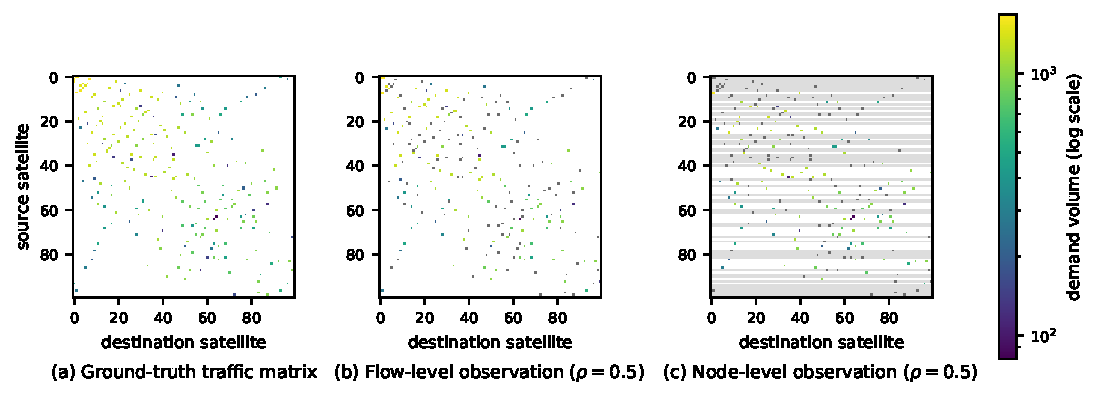
\includegraphics[width=\linewidth]{figures/sparse-tm.pdf}
    \caption{A ground-truth traffic matrix from the Starlink $22{\times}72$
    trace (150 busiest satellites shown) and its node-level sparse
    observation: white cells carry no traffic, gray rows are unmeasured
    source satellites, and colored cells are observed demands.}
    \label{fig:sparse-tm}
\end{figure}

\subsubsection{Problem Statement}
A key observation makes decision-making under unknown demands physically
executable: the decision variables are split \emph{ratios}, not absolute
volumes. Once installed in the forwarding plane, $r_i$ is applied
multiplicatively to whatever traffic actually arrives, so a decision for
demand $i$ requires no knowledge of $d_i$. Sparse-observation TE then
seeks a policy $\pi$ that maps the observable state to
split ratios for \emph{all} active demands,
\begin{equation}
    \{r_i\}_{i \in \mathcal{K}^t} = \pi\left(H^t, M, G^t\right),
    \label{eq:policy}
\end{equation}
maximizing the \emph{ground-truth} objective. Let
$f_{i,k}(\pi) = \tilde{r}_{i,k} \cdot d_i$ denote the flow actually
delivered on path $p_{i,k}$, where $\{\tilde{r}_i\}$ are the policy's
ratios after an optional repair step: ADMM
refinement with rounding under the throughput objective, and
conservation-preserving rebalancing under MLU, where the ratios are
already conservation-feasible by \cref{eq:conserve} but may still
overload individual links. Formally, for MLU minimization
\begin{equation}
    \min_{\pi} \;
    \mathbb{E}_t \Bigl[ \max_{e \in E^t}
        \frac{1}{c_e}\!\!\sum_{(i,k):\, e \in p_{i,k}}\!\! f_{i,k}(\pi)
    \Bigr],
    \label{eq:sparse-mlu}
\end{equation}
and, for the throughput variant,
\begin{equation}
    \max_{\pi} \;
    \mathbb{E}_t \Bigl[ \sum_{i \in \mathcal{K}^t} \sum_{k=1}^{\kappa}
        f_{i,k}(\pi) \Bigr],
    \label{eq:sparse-obj}
\end{equation}
where the expectations are over traffic and topology dynamics. Note that
the link loads in \cref{eq:sparse-mlu} are evaluated with the true
demands $d_i$: an unmeasured demand still consumes real capacity even
though the policy could not see it, so misjudging it inflates the
realized MLU. The problem
is a partially observable sequential decision problem: unlike
\crefrange{eq:mlu}{eq:nonneg}, where the same $D^t$ appears in both
the decision and the constraints, here the decision variables and the
evaluation live in different information sets: the policy acts on
$(O, M)$ only, while feasibility and performance are settled by the
hidden $D$. Intuitively, the policy is graded against an exam it never
gets to read in full.

\subsection{Solution Paradigm}
\label{sec:paradigm}

Three solution families exist for \cref{eq:sparse-mlu,eq:sparse-obj}.
\emph{Solve-with-zeros} plugs $O$ directly into the
LP in \crefrange{eq:mlu}{eq:nonneg}, implicitly assuming unmeasured
demands are zero; the resulting policy leaves no headroom on the links
that unmeasured traffic actually traverses, so the realized MLU can be far
above the optimum (and, under the throughput objective, unmeasured
demands are structurally starved). \emph{Two-stage} approaches first estimate $\hat{D}$ from $(H, M)$,
via interpolation, tensor completion, or compressive
sensing~\cite{vardi1996,zhang2003,zhang2009}, and then
solve the LP on $\hat{D}$; estimation is optimized for reconstruction error,
which is misaligned with allocation quality, and errors propagate un-damped
into the allocation. We instead adopt \emph{end-to-end learning}:
parameterize $\pi_\theta$ as a neural network and optimize $\theta$ directly
against the TE objective,
\begin{equation}
    \max_{\theta} \;
    \mathbb{E} \bigl[ R\bigl(\pi_\theta(H, M, G),\, D\bigr) \bigr],
    \label{eq:rl-obj}
\end{equation}
where $R$ is the TE objective evaluated on the true $D$: negative
realized MLU for \cref{eq:sparse-mlu}, or total satisfied demand
for \cref{eq:sparse-obj}. Since $R$
is non-differentiable through the capacity-constrained network and the true
$D$ is available only as a training-time signal, we
optimize \cref{eq:rl-obj} with multi-agent reinforcement learning, in
which each demand acts as an agent sharing $\theta$ and receives a
COMA-style marginal-contribution reward, followed by an
optional lightweight repair step at inference that relieves overloaded
links. This paradigm makes the observation
model in \cref{eq:obs} a property of the \emph{input}, and the optimization
target in \cref{eq:sparse-obj} a property of the \emph{training signal},
cleanly separating what the policy can see from what it is optimized for.
